\section{Issues}
\subsection{Fission Slack conversatie}
\label{sec:fission-slack-issue}
In afbeelding \ref{fig:fission-slack-issue-1} is de conversatie gevoerd op de Slack channel van het Fission project terug te vinden. Deze mensen hebben geprobeerd het probleem te verhelpen maar hebben ook geen oplossing kunnen aanreiken.
\begin{figure}
    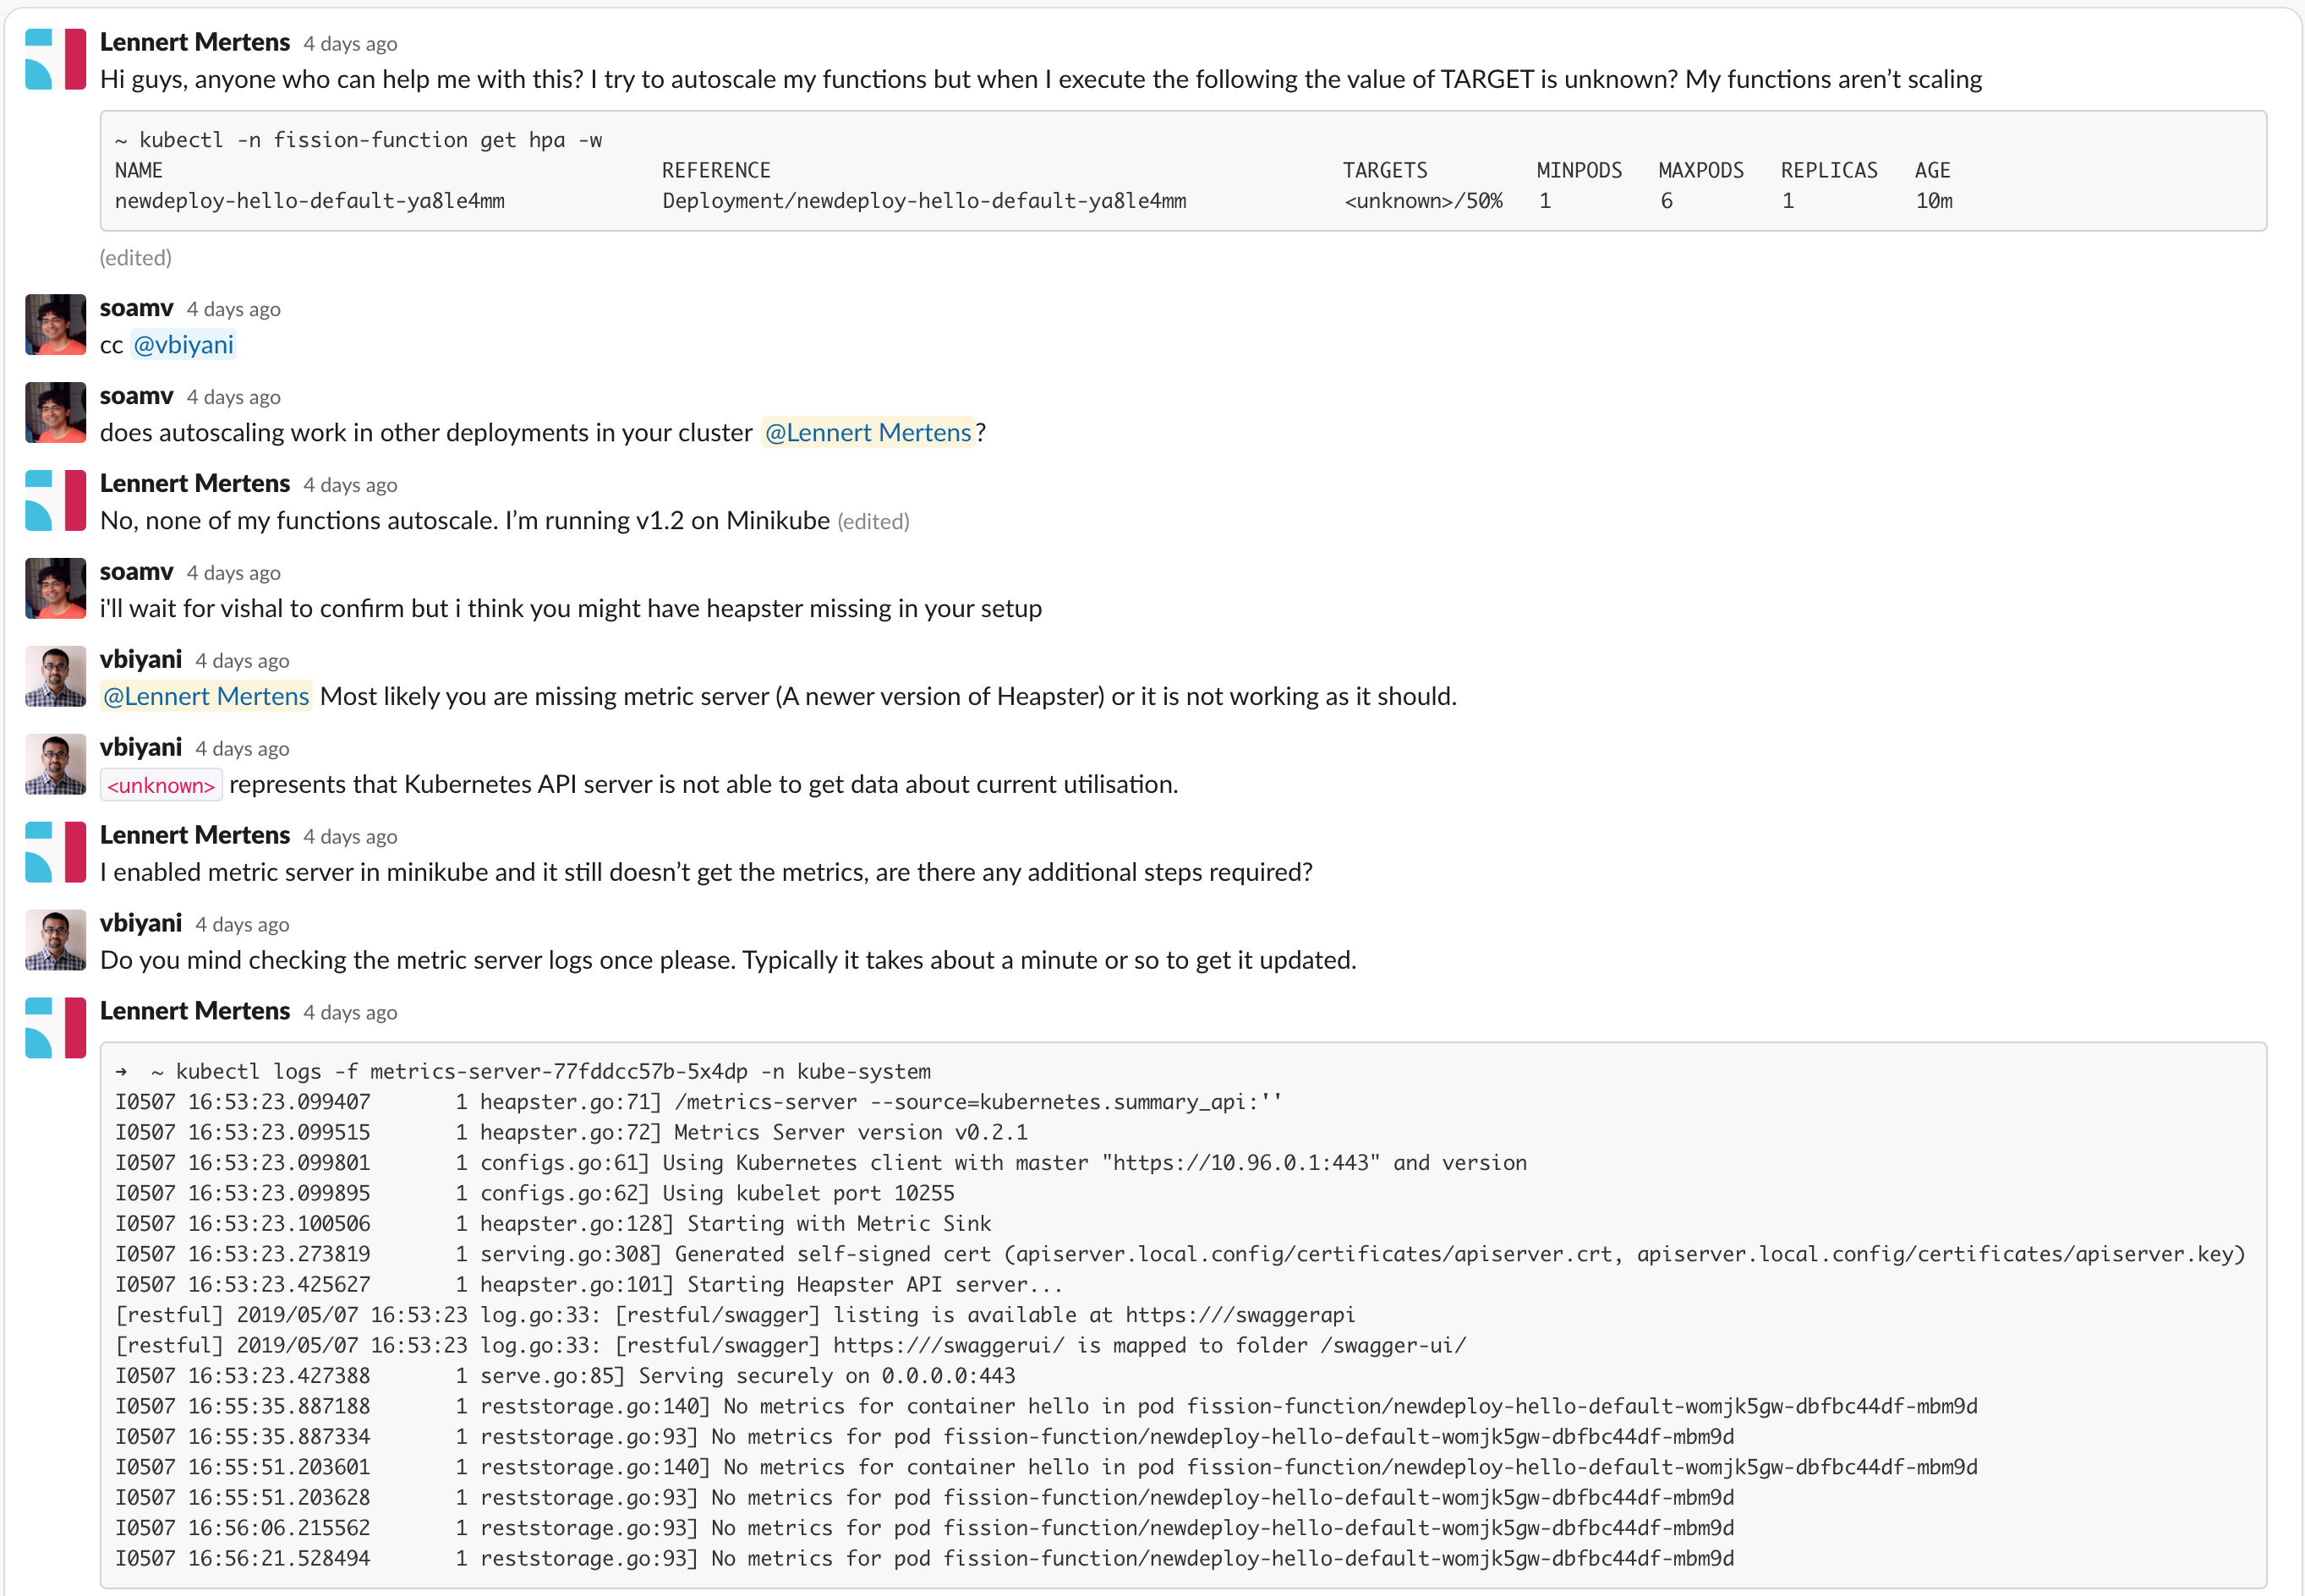
\includegraphics[width=1\textwidth]{img/fission-slack-issue-1.png}
     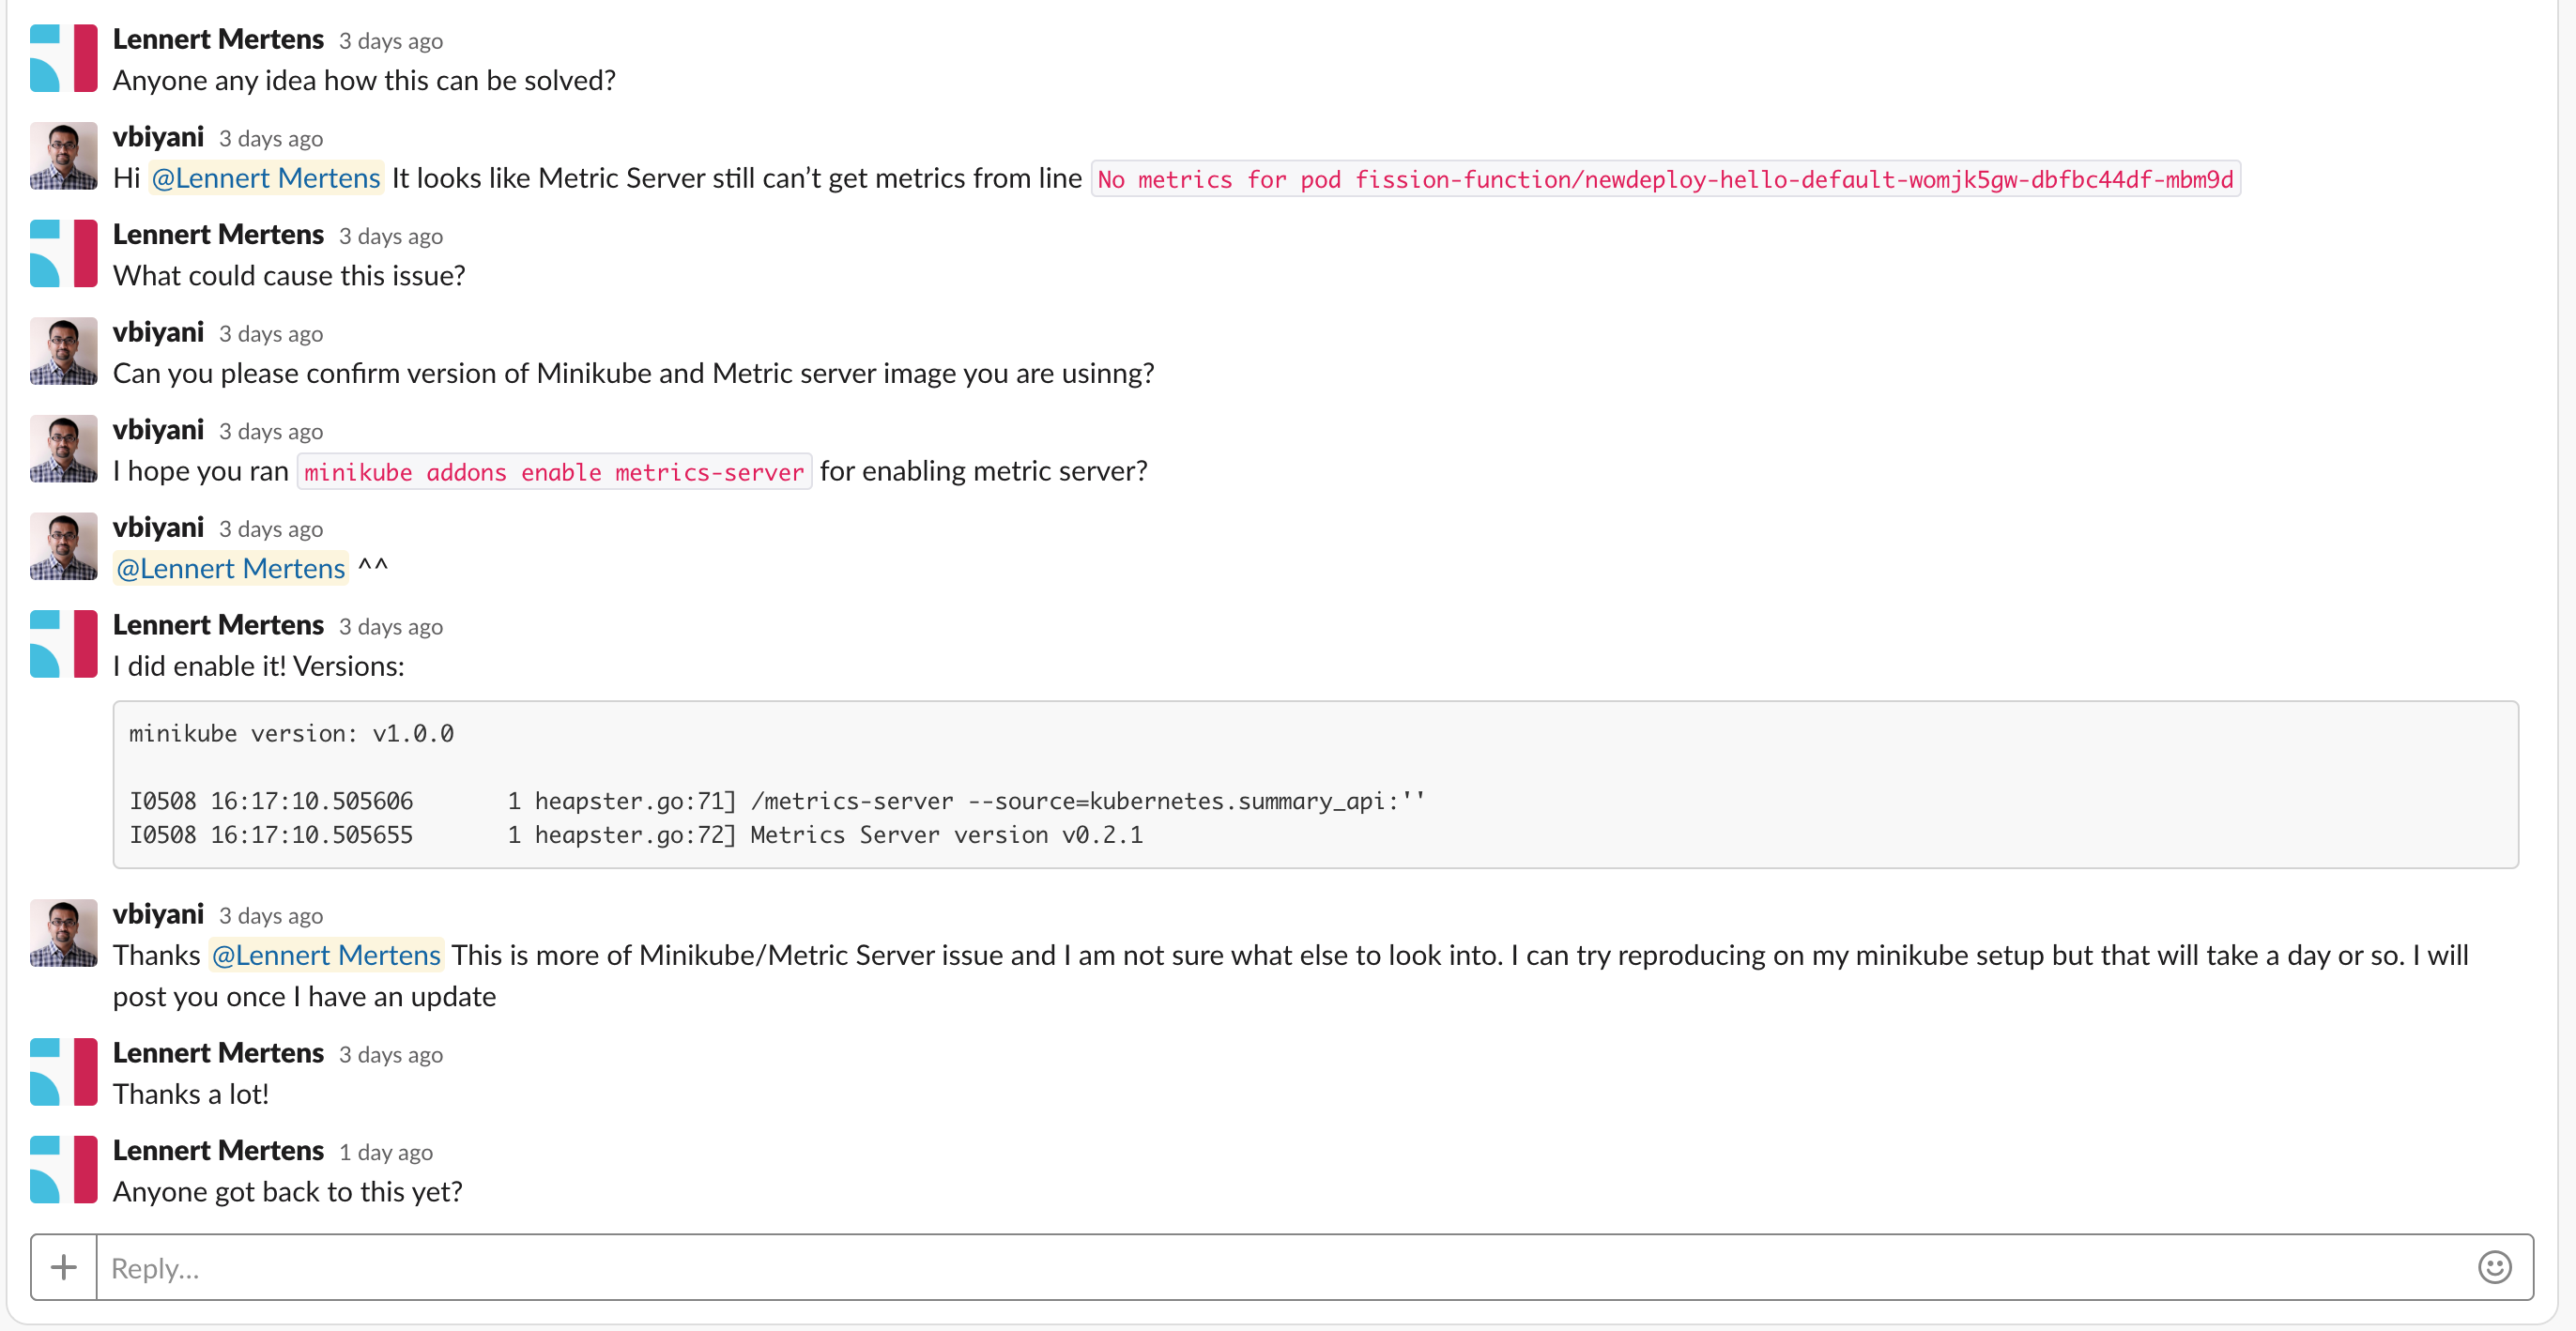
\includegraphics[width=1\textwidth]{img/fission-slack-issue-2.png}
    \caption{Fission Slack channel conversatie.}
    \label{fig:fission-slack-issue-1}  
\end{figure}

\subsection{Fission GitHub issue}
\label{sec:fission-github-issue}
Na troubleshooting en verder uitproberen werd er besloten een GitHub issue\footnote{https://github.com/fission/fission/issues/1182} aan te maken op het Fission project en de tegengekomen problemen te melden, dit kan anderen die hetzelfde probleem tegenkomen helpen. De issue werd gesloten en er werd ook geen concrete oplossing aangereikt.
\begin{figure}
    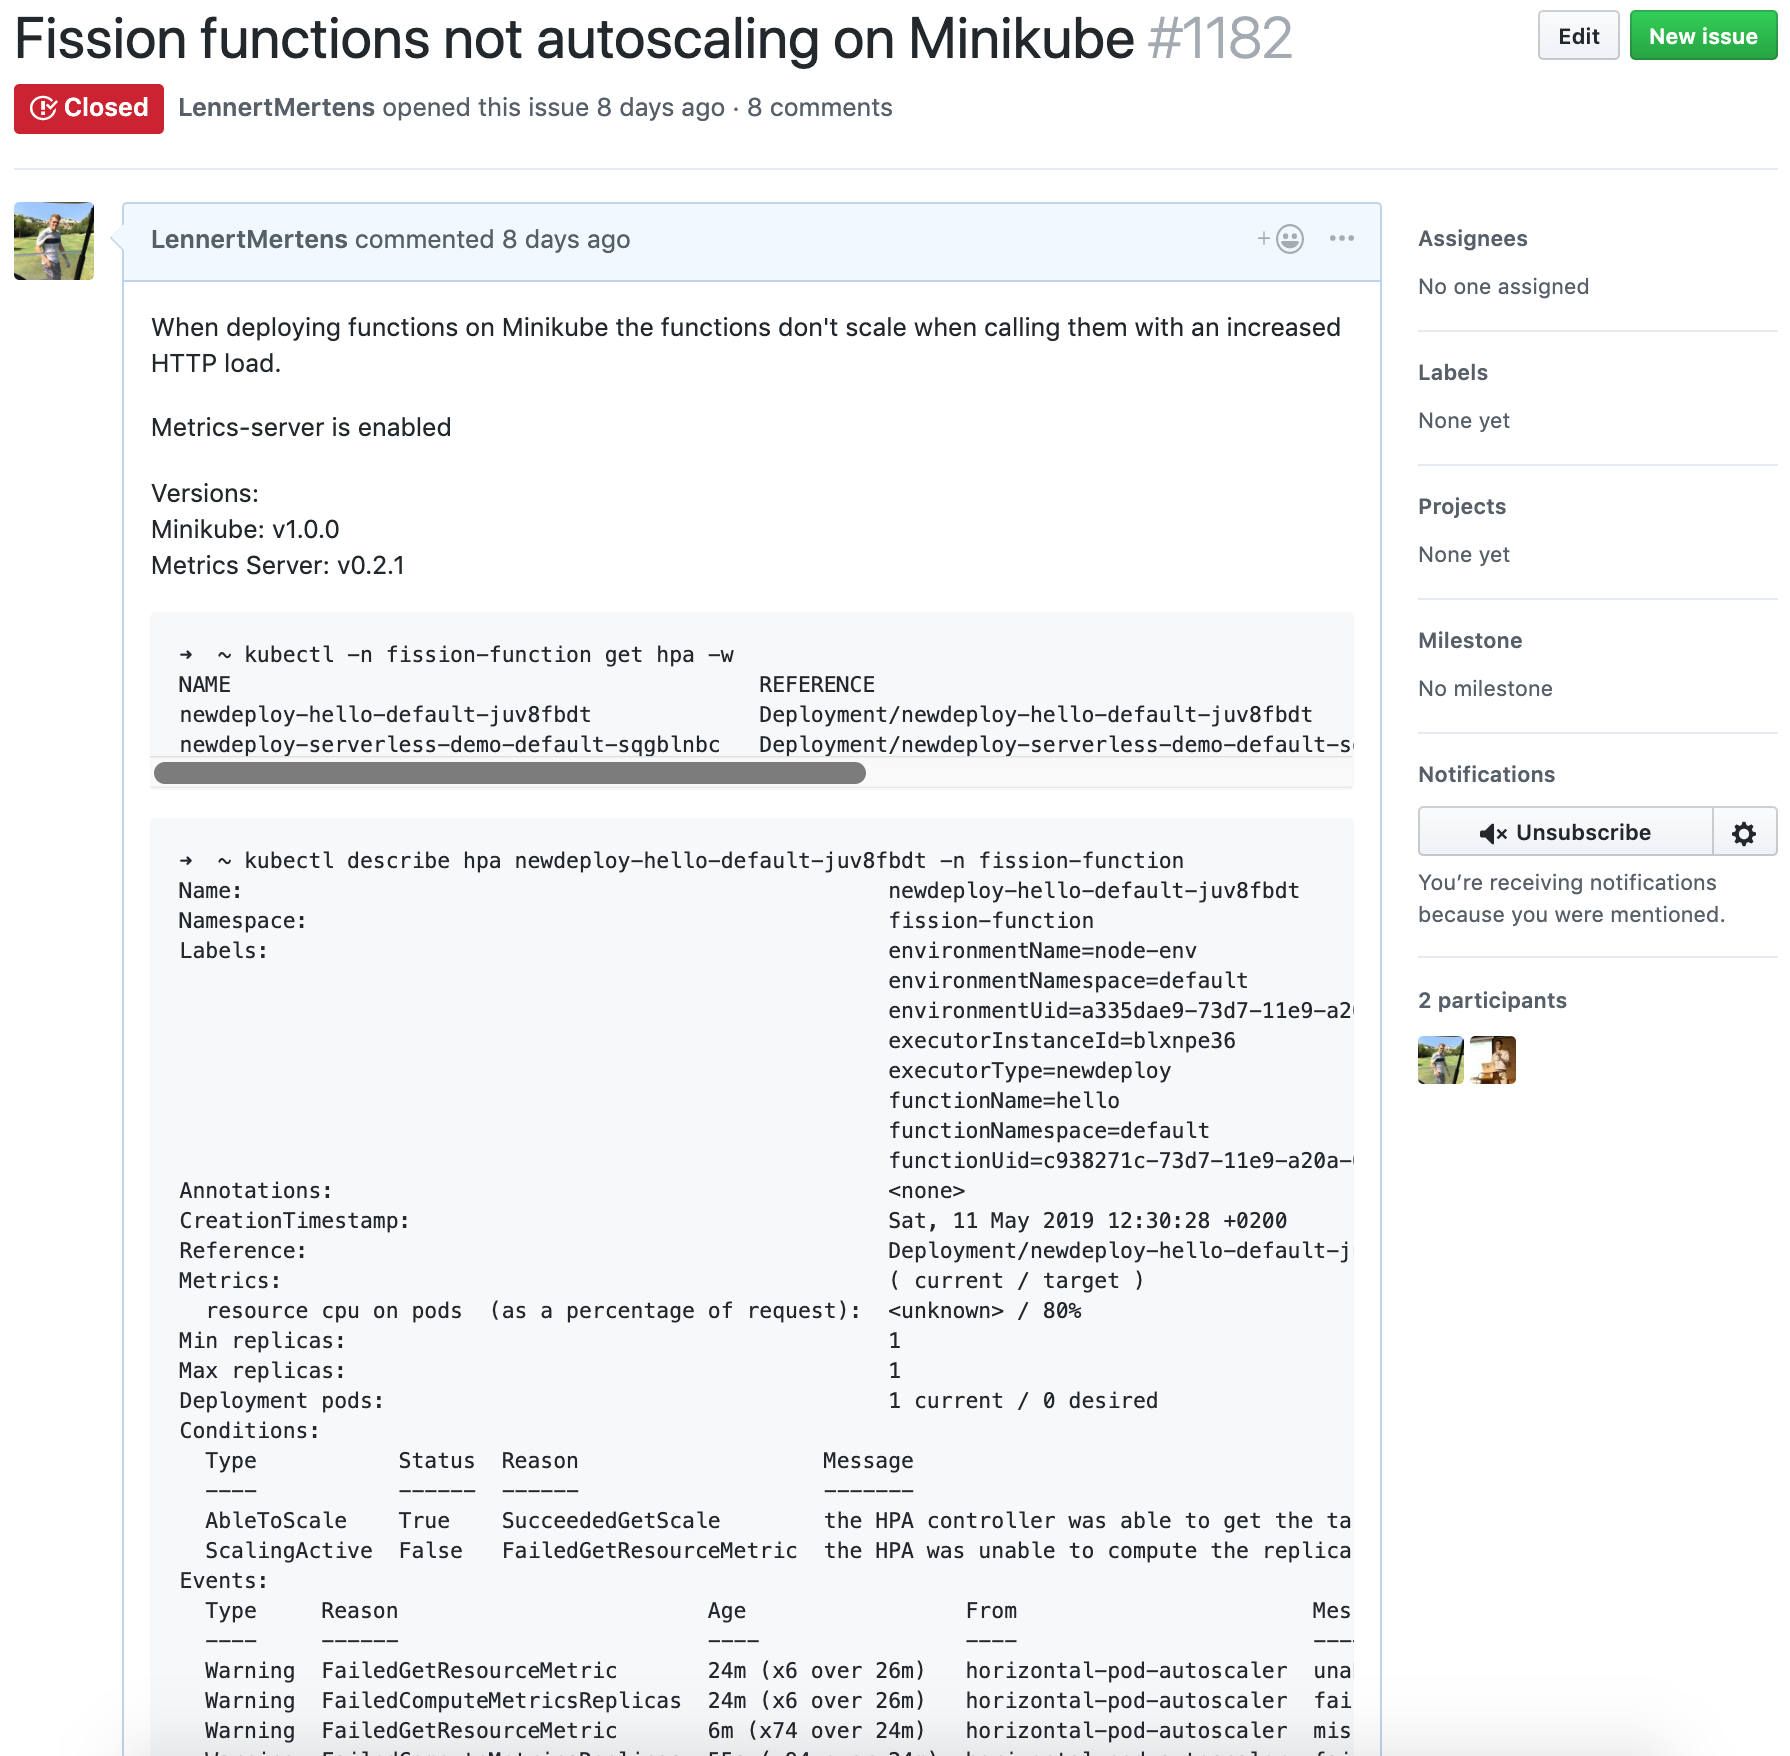
\includegraphics[width=1\textwidth]{img/fission-github-issue.png}
    \caption{Fission issue op GitHub.}
    \label{fig:fission-github-issue}  
\end{figure}